\newcommand{\fileInfectorTagResultsAucTable}{
    \begin{table}[H]
        \centering
        \begin{tabular}{|p{2,8cm}||p{2,8cm} p{2,8cm} p{2,8cm}|}
            \hline
            File-infector Tag & ALOHA & Joint Embedding & Proposed Model \\
            \hline
            AUC-ROC & 0.518$\pm$0.025 & 0.508$\pm$0.013 & \textBF{0.530$\pm$0.024} \\
            \hline
        \end{tabular}
        \caption{AUC-ROC (Area Under Curve) of the different models for the \textbf{File-infector Tag} prediction task. Results were aggregated over \textBF{3} training runs with different weight initializations and minibatch orderings. Best results are shown in \textbf{bold}.} \label{tab:fileInfectorTag_auc}
    \end{table}
}

\newcommand{\fileInfectorTagResultsAtFprTable}{
    \begin{center}
        \begin{longtable}[c]{|p{3,2cm}||p{1,8cm} p{1,8cm} p{1,8cm} p{1,8cm} p{1,8cm}|}
            \hline
            File-infector Tag & \multicolumn{5}{c|}{{FPR}} \\
            & $10^{-5}$ & $10^{-4}$ & $10^{-3}$ & $10^{-2}$ & $10^{-1}$ \\
            \hline
            \endfirsthead

            \caption*{\raggedright ...continued from previous page} \\
            \hline
            File-infector Tag & \multicolumn{5}{c|}{\textbf{FPR}} \\
            & $10^{-5}$ & $10^{-4}$ & $10^{-3}$ & $10^{-2}$ & $10^{-1}$ \\
            \hline
            \endhead

            \caption*{\raggedleft ...continued on next page} \\
            \endfoot

            \caption{Mean and standard deviation results (TPR, Accuracy, Recall, Precision and F1-Score) of the different models for the \textbf{File-infector Tag} prediction task at different \textbf{FPR}s (\textit{False Positive Rates}). Results were aggregated over \textBF{3} training runs with different weight initializations and minibatch orderings. Best results are shown in \textbf{bold}. Under \textbf{TPR} results are also presented the percentage reduction in mean detection error and in ROC curve standard deviation introduced by the \textit{Proposed Model} with respect to both \textit{ALOHA} model and \textit{Joint Embedding}.} \label{tab:fileInfectorTag_results_at_fpr} \\
            \endlastfoot

            \multicolumn{6}{|c|}{\textbf{TPR}} \\
            \hline
            ALOHA & 0.003$\pm$0.004 & 0.003$\pm$0.004 & \textBF{0.005$\pm$0.007} & 0.017$\pm$0.006 & 0.117$\pm$0.039 \\
            Joint Embedding & \textBF{0.003$\pm$0.002} & \textBF{0.003$\pm$0.002} & 0.003$\pm$0.002 & 0.011$\pm$0.006 & 0.117$\pm$0.023 \\
            Proposed Model & 0.002$\pm$0.002 & 0.002$\pm$0.002 & 0.003$\pm$0.002 & \textBF{0.020$\pm$0.008} & \textBF{0.128$\pm$0.021} \\
            \hline
            Error Reduction wrt \newline ALOHA & -0.1\% & -0.1\% & -0.2\% & 0.3\% & 1.2\% \\
            Error Reduction wrt \newline Joint Embedding & -0.1\% & -0.1\% & 0.0\% & 0.9\% & 1.2\% \\
            \hline
            Std Reduction wrt \newline ALOHA & 50.0\% & 50.0\% & 71.4\% & -33.3\% & 46.2\% \\
            Std Reduction wrt \newline Joint Embedding & 0.0\% & 0.0\% & 0.0\% & -33.3\% & 8.7\% \\
            \hline
            \multicolumn{6}{|c|}{\textbf{Accuracy}} \\
            \hline
            ALOHA & \textBF{0.912$\pm$0.000} & \textBF{0.912$\pm$0.000} & 0.911$\pm$0.001 & 0.904$\pm$0.000 & 0.831$\pm$0.004 \\
            Joint Embedding & \textBF{0.912$\pm$0.000} & \textBF{0.912$\pm$0.000} & \textBF{0.912$\pm$0.000} & 0.905$\pm$0.002 & 0.831$\pm$0.002 \\
            Proposed Model & \textBF{0.912$\pm$0.000} & \textBF{0.912$\pm$0.000} & 0.911$\pm$0.000 & \textBF{0.905$\pm$0.001} & \textBF{0.832$\pm$0.001} \\
            \hline
            \multicolumn{6}{|c|}{\textbf{Recall}} \\
            \hline
            ALOHA & 0.003$\pm$0.004 & 0.003$\pm$0.004 & \textBF{0.005$\pm$0.007} & 0.017$\pm$0.006 & 0.117$\pm$0.039 \\
            Joint Embedding & \textBF{0.003$\pm$0.002} & \textBF{0.003$\pm$0.002} & 0.003$\pm$0.002 & 0.011$\pm$0.006 & 0.117$\pm$0.023 \\
            Proposed Model & 0.002$\pm$0.002 & 0.002$\pm$0.002 & 0.003$\pm$0.002 & \textBF{0.020$\pm$0.008} & \textBF{0.128$\pm$0.021} \\
            \hline
            \multicolumn{6}{|c|}{\textbf{Precision}} \\
            \hline
            ALOHA & \textBF{1.000$\pm$0.000} & \textBF{1.000$\pm$0.000} & 0.200$\pm$0.283 & 0.142$\pm$0.041 & 0.101$\pm$0.030 \\
            Joint Embedding & \textBF{1.000$\pm$0.000} & \textBF{1.000$\pm$0.000} & \textBF{0.500$\pm$0.408} & 0.112$\pm$0.061 & 0.102$\pm$0.018 \\
            Proposed Model & \textBF{1.000$\pm$0.000} & \textBF{1.000$\pm$0.000} & 0.250$\pm$0.204 & \textBF{0.165$\pm$0.059} & \textBF{0.111$\pm$0.016} \\
            \hline
            \multicolumn{6}{|c|}{\textbf{F1 Score}} \\
            \hline
            ALOHA & 0.006$\pm$0.009 & 0.006$\pm$0.009 & \textBF{0.009$\pm$0.013} & 0.030$\pm$0.010 & 0.109$\pm$0.034 \\
            Joint Embedding & \textBF{0.006$\pm$0.004} & \textBF{0.006$\pm$0.004} & 0.006$\pm$0.004 & 0.020$\pm$0.011 & 0.109$\pm$0.020 \\
            Proposed Model & 0.003$\pm$0.004 & 0.003$\pm$0.004 & 0.006$\pm$0.004 & \textBF{0.036$\pm$0.014} & \textBF{0.119$\pm$0.018} \\
            \hline
        \end{longtable}
    \end{center}
}

\newcommand{\fileInfectorTagResultsSummaryTable}{
    \begin{table}[H]
        \centering
        \begin{tabular}{|p{3,2cm}||p{1,8cm} p{1,8cm} p{1,8cm} p{1,8cm} p{1,8cm}|}
            \hline
            \multicolumn{6}{|c|}{File-infector Tag (at FPR $=1\%$)} \\
            \hline
            Model & TPR & Accuracy & Precision & Recall & F1 score \\
            \hline
            ALOHA & 0.017$\pm$0.006 & 0.904$\pm$0.000 & 0.142$\pm$0.041 & 0.017$\pm$0.006 & 0.030$\pm$0.010 \\
            Joint Embedding & 0.011$\pm$0.006 & 0.905$\pm$0.002 & 0.112$\pm$0.061 & 0.011$\pm$0.006 & 0.020$\pm$0.011 \\
            Proposed Model & \textBF{0.020$\pm$0.008} & \textBF{0.905$\pm$0.001} & \textBF{0.165$\pm$0.059} & \textBF{0.020$\pm$0.008} & \textBF{0.036$\pm$0.014} \\
            \hline
        \end{tabular}
        \caption{Summary of the mean and standard deviation results of the different models for the \textbf{File-infector Tag} prediction task at \textbf{FPR} $=1\%$. Results were aggregated over \textBF{3} training runs with different weight initializations and minibatch orderings. Best results are shown in \textbf{bold}.} \label{tab:fileInfectorTag_result_summary}
    \end{table}
}

\newcommand{\fileInfectorTagRocAloha}{
    \begin{figure}[H]
        \centering
        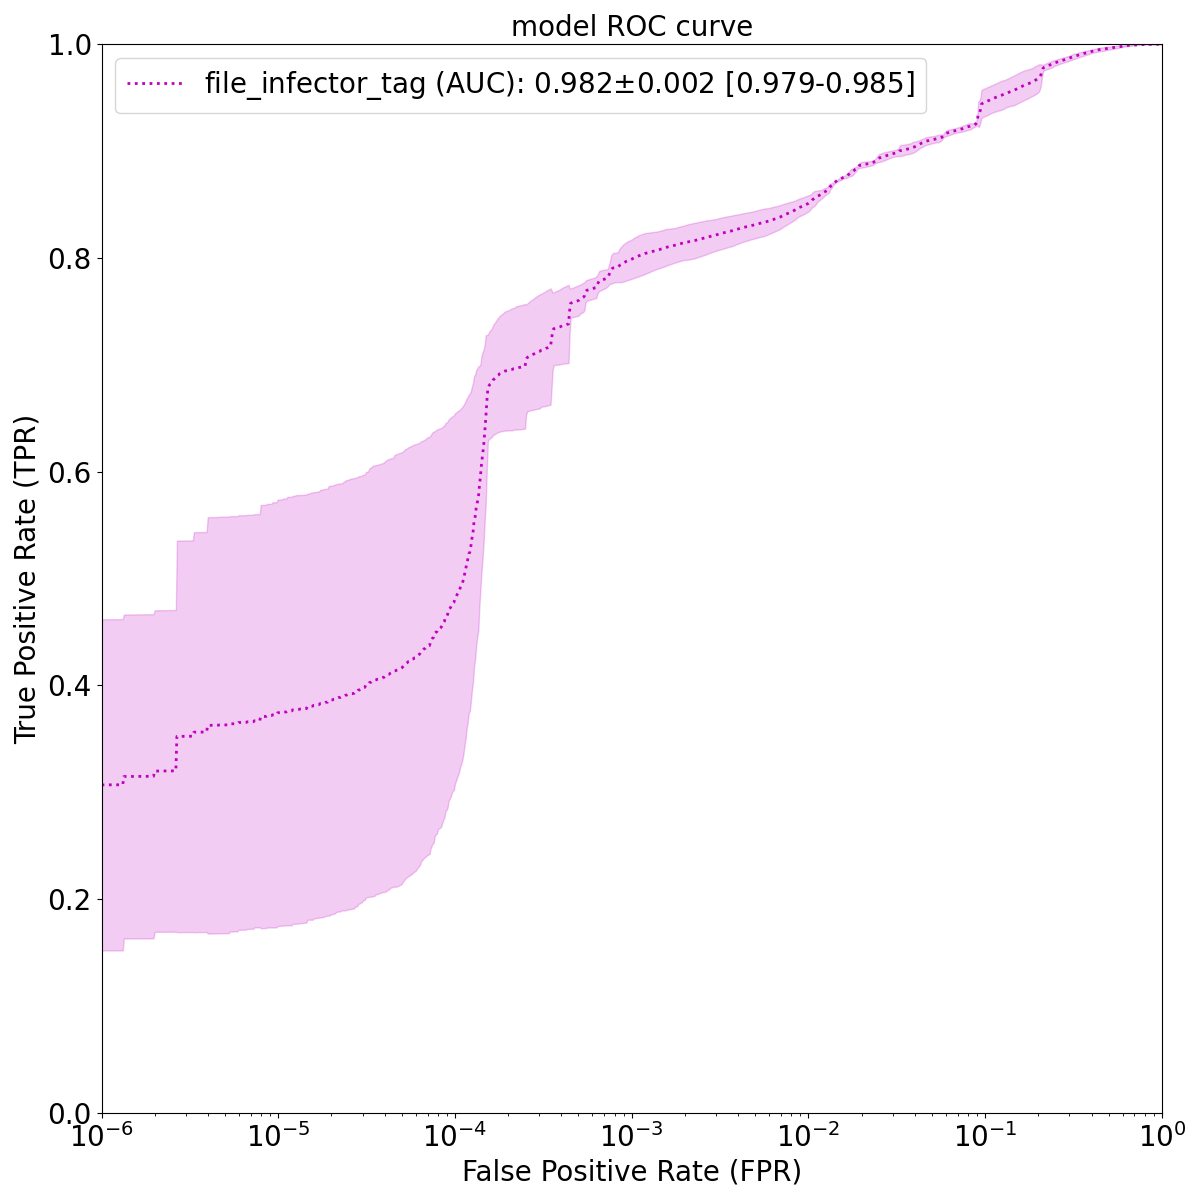
\includegraphics[width=0.8\textwidth]{./results/file_infector_tag_roc_aloha.png}
        \vspace*{-1cm}
        \caption{ROC curve and AUC statistics of \textBF{ALOHA} model for the \textbf{File-infector Tag}. The line represents the \textit{mean} TPR at a given FPR, while the shaded region represents the \textit{standard deviation}. Statistics were computed over \textBF{3} training runs, each with random parameter initialization.}
        \label{fig:fileInfectorTagRocAloha}
    \end{figure}
}

\newcommand{\fileInfectorTagRocJointEmbedding}{
    \begin{figure}[H]
        \centering
        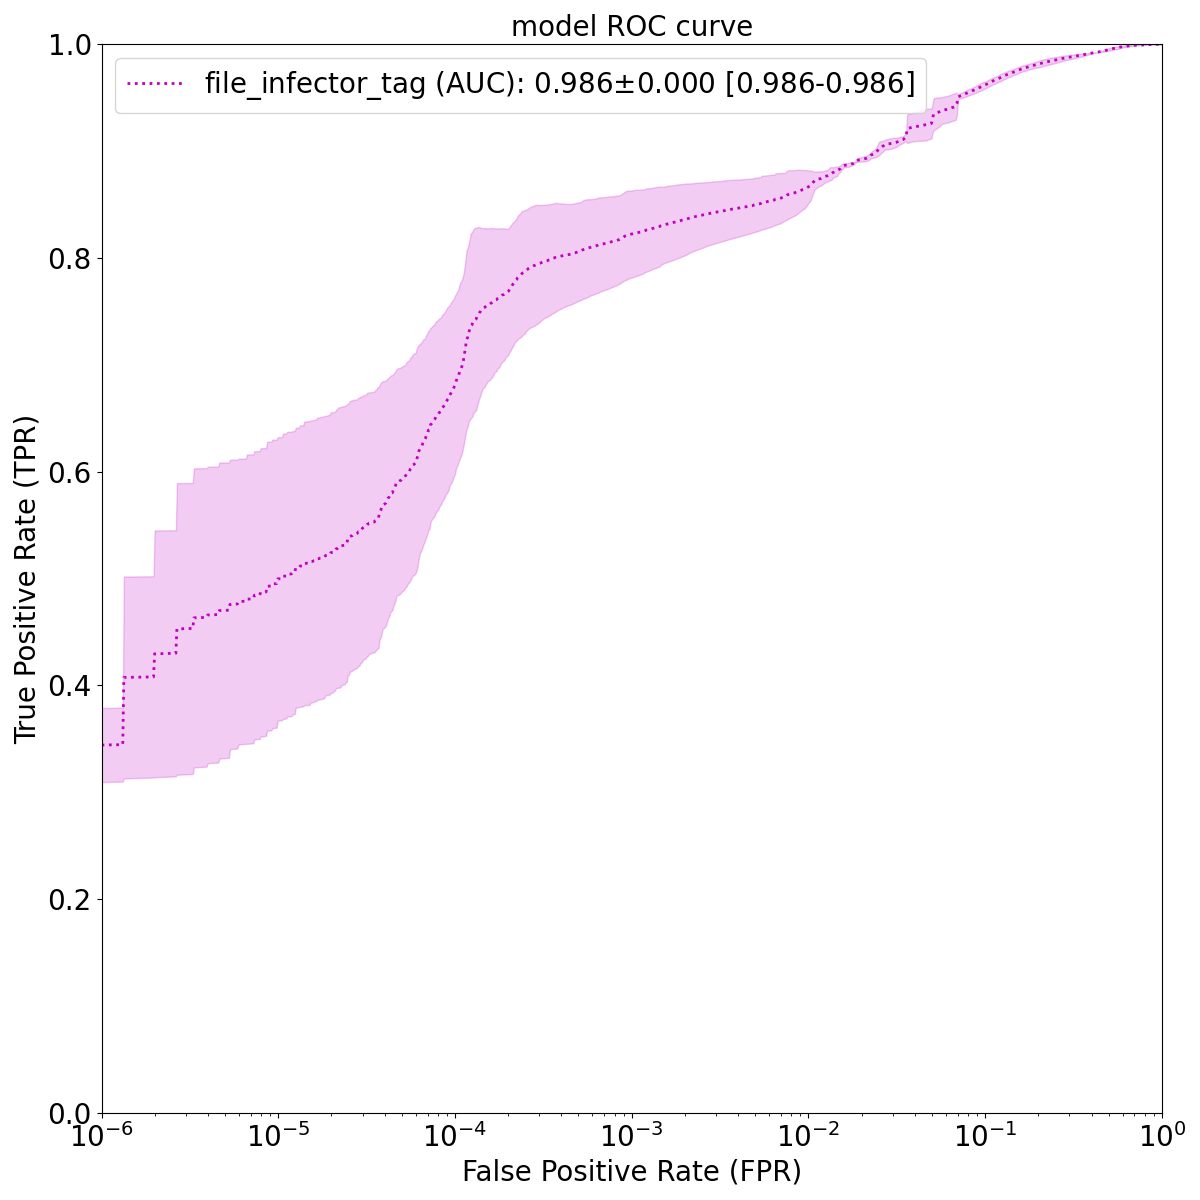
\includegraphics[width=0.8\textwidth]{./results/file_infector_tag_roc_jointEmbedding.png}
        \vspace*{-1cm}
        \caption{ROC curve and AUC statistics of \textBF{Joint Embedding} model for the \textbf{File-infector Tag}. The line represents the \textit{mean} TPR at a given FPR, while the shaded region represents the \textit{standard deviation}. Statistics were computed over \textBF{3} training runs, each with random parameter initialization.}
        \label{fig:fileInfectorTagRocJointEmbedding}
    \end{figure}
}

\newcommand{\fileInfectorTagRocProposedMethod}{
    \begin{figure}[H]
        \centering
        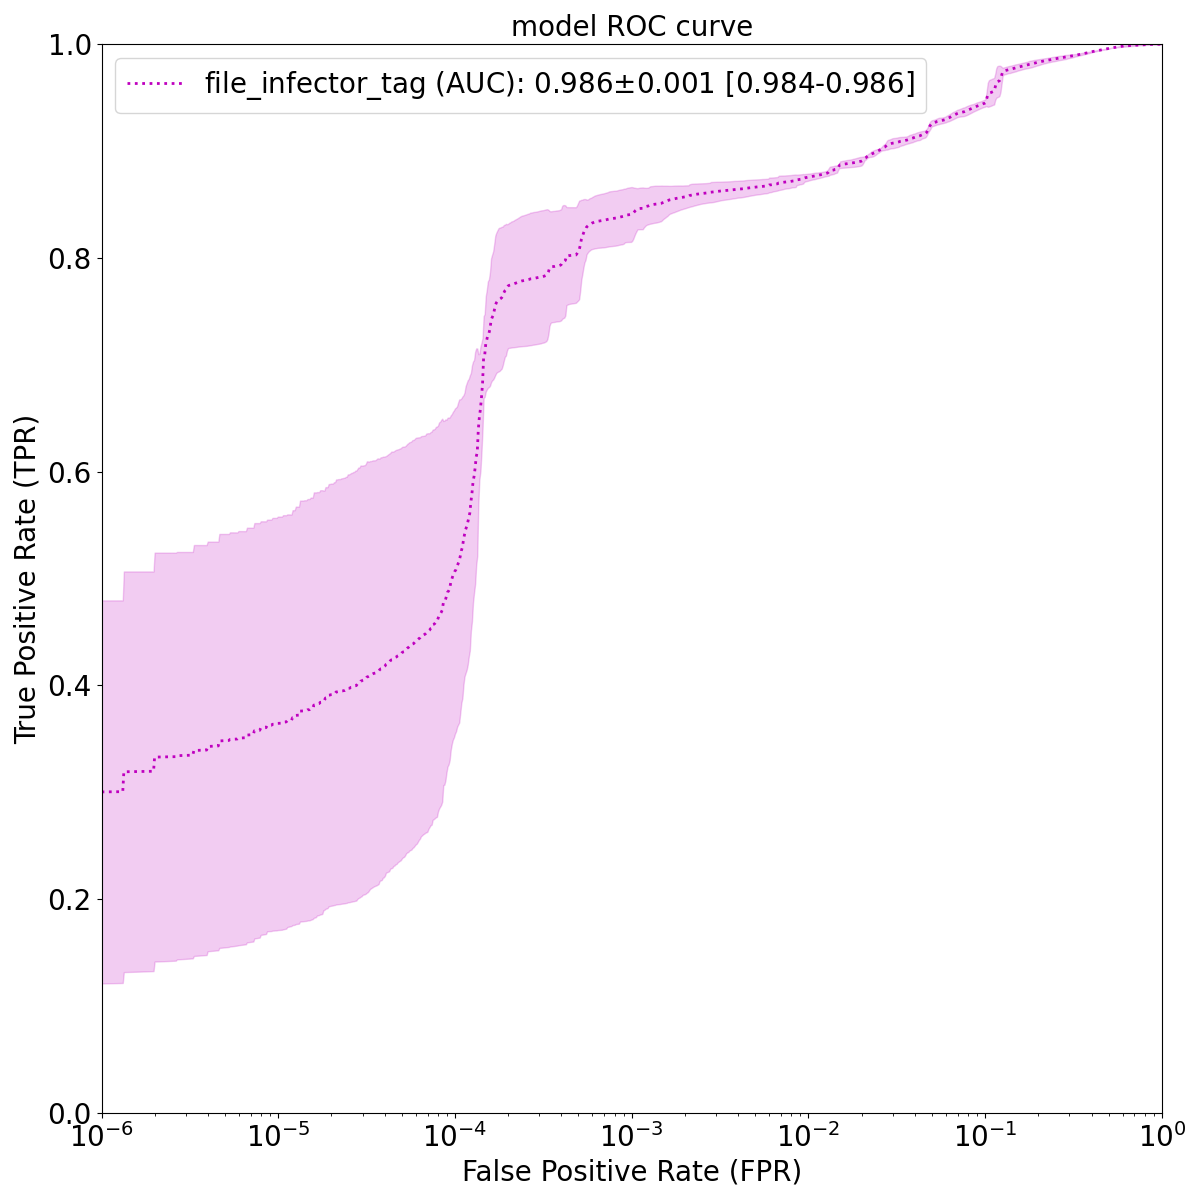
\includegraphics[width=0.8\textwidth]{./results/file_infector_tag_roc_proposedModel.png}
        \vspace*{-1cm}
        \caption{ROC curve and AUC statistics of \textBF{Proposed Model} for the \textbf{File-infector Tag}. The line represents the \textit{mean} TPR at a given FPR, while the shaded region represents the \textit{standard deviation}. Statistics were computed over \textBF{3} training runs, each with random parameter initialization.}
        \label{fig:fileInfectorTagRocProposedModel}
    \end{figure}
}
